\section{Theory}

A polarizing microscope is used for the experiments in this report. In this section the basic principles of a polarizing microscope and the theory that is used for the experiments are described.

\begin{wrapfigure}{r}{0.3\textwidth}
    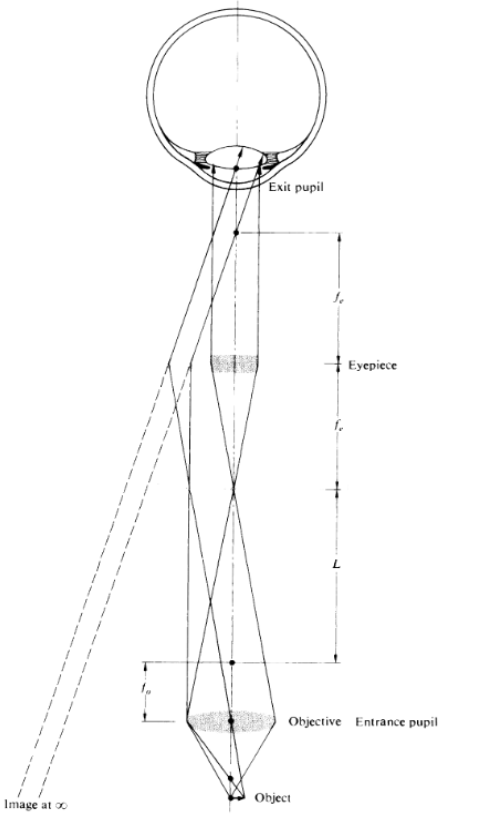
\includegraphics[width=0.25\textwidth]{afbeeldingen/compound_microscope.png}
  	\caption{Schematic drawing of a compound microscope. $f_{e}$ and $f_{o}$ correspond to respectively to the focussing distance of the eyepiece and objective. This figure was apdapted from \cite{hecht}.}
  	\label{fig_compound_microscope}
\end{wrapfigure} 

\subsubsection{Microscopy}

Most modern microscopes are compound microscopes. These type of microscopes can achieve a relatively high angular magnification for nearby objects (Hecht, 2016). For this system, an objective, being the entrance pupil of the system, creates a real inverted, magnified image. The eyepiece creates a virtual images with greater magnification which can be viewed comfortably. The total magnification of the microscope is the product of the individual magnifications of the eyepiece and objective (Hecht, 2016). See figure \ref{fig_compound_microscope} for a schematic drawing of a basic compound microscope. 



\subsubsection{CCD recording}
In this experiment it was chosen to use a CCD camera to record the imaged from the microscope. To measure distances in a sample it is possible to convert a distance in pixels, $n_{pixels}$, to physical unit such as meters. For this, we need a conversion factor that gives the length in meters per pixel, $l_{pixel}$. The physical distance, $d_{physical}$ can easily be calculated using equation \ref{eq_distance}.

\begin{equation}
	\label{eq_distance}
	d_{physical} = l_{pixel} \cdot n_{pixels}
\end{equation}








\begin{comment}
In  theTheorie  (Theory)  chapter,  you  describe  all  (and  only!)  the  theory needed  to  understand  and  interpret the experiments  in  the  remainder  of  the  report.    Explain  to  the  reader  why  a  piece  of  theory  is  relevant  for  your  research.  Equations  should  be  numbered.  If  an  equation  cannot  be  assumed  to  be  generally known by the readers (see General Hint 2 for the level of the audience), you should provide a reference to an accessible textbook or article (so not to the RP manual, lecture notes, Wikipedia etc.). In general, try to avoid referring to websites, online data or Wikipedia.
\end{comment}